%%!TEX root = dissertation.tex

\chapter{The SpiCE Corpus}
\label{ch:Corpus}

\section{Introduction}\label{ch2:sec:introduction}
Most of our knowledge about spoken language and speech processing comes from monolingual individuals producing scripted speech in laboratory settings. Monolingual lab speech allows for researchers to exercise tight control over the linguistic backgrounds of the speakers and the linguistic material (e.g. reading or repeating sounds, words, or sentences). While highly informative, these controlled monolingual speech samples are not representative of spoken language in the real world. Multilingualism is the norm, not the exception, and individuals regularly make creative linguistic choices. 

Crucially, corpus-based research with conversational or spontaneous speech is important in the fields of phonetics and psycholinguistics, as the research conclusions drawn from corpus and lab-based experiments do not always coincide \citep{gahl_2012_reduce}. Conversational speech allows for a more accurate empirical description of spoken language, as it represents more realistic and natural productions than scripted laboratory speech, even compared to scripted connected speech. Conversational speech also crucially permits for field testing of speech production theories \citep{bell_2009_predictability, gahl_2012_reduce} in their natural habitats. 

The discrepancies between results for conversational and lab speech have been found for monolingual (English) speech, but are likely be found with bilingual speech as well. Resources to query bilingual conversational speech are limited, however, as the necessary resources permitting this type of inquiry are rare. As a step towards filling this gap, this chapter introduces the \textbf{SpiCE} corpus of conversational bilingual \textbf{Sp}eech \textbf{i}n \textbf{C}antonese and \textbf{E}nglish. This open-access corpus was explicitly developed with phonetic bilingualism research in mind. The corpus design is based on key aspects of widely used existing corpora, such as the Buckeye corpus of conversational speech \citep{pitt_2005_buckeye}. It crucially includes speech from the same individual in more than one language, as is the case in the Bangor corpora of Spanish-English, Welsh-English, and Welsh-Spanish bilingual speech \citep{deuchar_2014_corpora}, but with a more controlled recording setup, allowing for more nuanced acoustic-phonetic measurements. 

The primary motivation for collecting this corpus was to have comparable high-quality recordings of conversational speech from early bilinguals in two languages, which in turn enables large scale phonetic analysis on a within-speaker basis.\footnote{SpiCE is a large speech corpus for the type of speech involved, and is comparable in size to the widely used Buckeye corpus \citep{pitt_2005_buckeye}. Larger speech corpora tend to comprise existing recordings of broadcasters, phone conversations, or read speech. While these types of speech corpora are certainly useful, they are designed for different purposes.} To our knowledge, this type of resource does not yet exist for any pair of languages, much less for a typologically distinct pair like Cantonese (Sino-Tibetan) and English (Indo-European). Furthermore, Cantonese is a relatively understudied language, despite there being approximately 55 million native speakers around the world \citep{matthews_2013_cantonese}, though this is changing with new corpora \citep{luke_2015_hkc,leung_2001_hkcac,winterstein_2020_cantomap,alderete_2019_tone} and tools \citep{lee_2018_pycantonese,yau_2019_pyjyutping}.

This chapter provides a detailed overview of the corpus design and collection procedures, a description of the speakers, and the transcription and annotation pipeline. It concludes with descriptive statistics. 

\begin{table}[!htbp]
\begin{center}
\begin{tabular}{ccccccc}
\toprule
  % & & & &                & \multicolumn{2}{c}{\textbf{Age of Acquisition}} \\
\textbf{No.} & \textbf{ID} & \textbf{Order} & \textbf{Age} & \textbf{Gender} & \textbf{English AoA} & \textbf{Cantonese AoA} \\
\midrule
1 & VF19A & E $\rightarrow$ C & 19  & F & 0   & 0 \\
2 & VF19B & E $\rightarrow$ C & 19  & F & 0   & 0 \\
3 & VF19C & E $\rightarrow$ C & 19  & F & 3   & 0 \\
4 & VF19D & C $\rightarrow$ E & 19  & F & 2   & 0 \\
5 & VF20A & C $\rightarrow$ E & 20  & F & 4   & 0 \\
6 & VF20B & C $\rightarrow$ E & 20  & F & 5   & 0 \\
7 & VF21A & E $\rightarrow$ C & 21  & F & 0   & 0 \\
8 & VF21B & C $\rightarrow$ E & 21  & F & 3   & 0 \\
9 & VF21C & C $\rightarrow$ E & 21  & F & 4   & 0 \\
10  & VF21D & E $\rightarrow$ C & 21  & F & 0   & 0 \\
11  & VF22A & C $\rightarrow$ E & 22  & F & 0   & 0 \\
12  & VF23B & E $\rightarrow$ C & 23  & F & 2   & 0 \\
13  & VF23C & C $\rightarrow$ E & 23  & F & 0   & 0 \\
14  & VF26A & C $\rightarrow$ E & 26  & F & 0   & 0 \\
15  & VF27A & E $\rightarrow$ C & 27  & F & 0   & 0 \\
16  & VF32A & C $\rightarrow$ E & 32  & F & 3   & 0 \\
17  & VF33B & C $\rightarrow$ E & 33  & F & 0   & 0 \\
18  & VM19A & E $\rightarrow$ C & 19  & M & 0   & 0 \\
19  & VM19B & C $\rightarrow$ E & 19  & M & 2   & 0 \\
20  & VM19C & E $\rightarrow$ C & 19  & M & 0   & 0 \\
21  & VM19D & C $\rightarrow$ E & 18  & M & 1   & 1 \\
22  & VM20B & E $\rightarrow$ C & 20  & M & 0   & 0 \\
23  & VM21A & E $\rightarrow$ C & 21  & M & 0   & 0 \\
24  & VM21B & E $\rightarrow$ C & 21  & M & 0   & 0 \\
25  & VM21C & C $\rightarrow$ E & 21  & M & 0   & 0 \\
26  & VM21D & C $\rightarrow$ E & 21  & M & 0   & 0 \\
27  & VM21E & C $\rightarrow$ E & 21  & M & 5   & 0 \\
28  & VM22A & C $\rightarrow$ E & 22  & M & 4   & 0 \\
29  & VM22B & E $\rightarrow$ C & 22  & M & 0   & 0 \\
30  & VM23A & E $\rightarrow$ C & 23  & M & 0   & 0 \\
31  & VM24A & E $\rightarrow$ C & 24  & M & 3   & 0 \\
32  & VM25A & E $\rightarrow$ C & 25  & M & 4   & 0 \\
33  & VM25B & E $\rightarrow$ C & 25  & M & 0   & 0 \\
34  & VM34A & C $\rightarrow$ E & 34  & M & 0   & 0 \\
\bottomrule

\end{tabular}
\caption{Basic participant information, including age, gender, age of acquisition (AoA), and the order the interviews occurred.}
\label{ch2:tab:participants}
\end{center}
\end{table}

\section{Corpus design and creation}\label{ch2:sec:design}

This section provides detail about the speakers (Section~\ref{ch2:subsec:participants}), the procedures used to ensure high-quality recordings (Section~\ref{ch2:subsec:setup}), and the three tasks that each participant completed in both Cantonese and English (Section~\ref{ch2:subsec:procedure}). 

Data collection took place between November 2018 and March 2020. Orthographic transcription began shortly after the first interview was recorded, and was completed in April 2021.

\subsection{Participants}\label{ch2:subsec:participants} 
The recordings in this corpus will comprise the speech of 34 early Cantonese-English bilinguals, 17 of which are female. At the time of submission, ten of 17 male participants had been recorded. All participants were between the ages of 19 and 35 (inclusive), reported normal speech and hearing, and resided in Vancouver, Canada at the time of recording. All participants in the study completed an extensive language background questionnaire, which included questions about language background, proficiency, use, and general demographics. A summary of language background information for all recorded speakers in the corpus is provided in Table~\ref{ch2:tab:participants}. A more comprehensive language background summary will be released along with the corpus audio and transcripts (see Section~\ref{ch2:sec:releases} for more details about releases).

Definitions of bilingualism are highly variable in the literature, as there are many different types of bilinguals \citep{amengual_2017_type}. For the purposes of this corpus, an early bilingual is someone who acquired both Cantonese and English before starting primary school (approximately age 5), and reports consistent use of both languages since that time. It is important to highlight that the Cantonese-English bilingual community in Vancouver (and Canada more generally) is incredibly diverse, both in terms of dialects spoken, as well as the regions from which families originally emigrated \citep{yu_2013_diaspora}. Furthermore, given the prevalence of Cantonese in Vancouver \citep{statistics_2017_proportion}, and longevity of the community \citep{yu_2013_diaspora}, immigration from other Cantonese-speaking areas continues today. 

This corpus reflects the diverse nature of Cantonese-English bilingualism in Vancouver, as it includes Canadian-born heritage speakers, recent immigrants from Hong Kong, as well as Cantonese speakers from other parts of the Cantonese diaspora. As a result, while all speakers are early bilinguals, various dialects are represented. The most well-represented dialect is Hong Kong Cantonese, as 20 of 27 participants report having at least one caretaker from Hong Kong (14 report only Hong Kong born caretakers). 

\subsection{Recording Setup}\label{ch2:subsec:setup}
Recording took place in a quiet room in the linguistics laboratory building at the University of British Columbia in Vancouver, Canada. Two Cantonese-English bilingual research assistants (the third and fourth authors) and the participant were seated around a table. The interviewer was a female Cantonese-English bilingual from Metro Vancouver. The recording process was monitored by a male Cantonese-English bilingual from Hong Kong, who moved to Vancouver to attend university. The interviewer and participant were outfitted with AKG C520 head-mounted microphones positioned approximately 3 cm from the corner of the mouth. The microphones were connected to separate channels on a Sound Devices USBPre2 Portable Audio Interface. Stereo recordings were made with Audacity 2.2.2 \citep{audacity_2018_audio} on a PC laptop, and saved according to best archival practices, with a 44.1 kHz sampling rate, and 24-bit resolution.

\subsection{Recording Procedure}\label{ch2:subsec:procedure}
Upon arrival, participants were provided with an overview of the recording session procedures, and informed of the corpus publication process. Subsequently, participants were asked to provide written consent. Upon consent, participants completed a session in English, and a session in Cantonese. The order of languages was counterbalanced across participants (see Table~\ref{ch2:tab:participants}). Each session consisted of three tasks\textemdash sentence reading, storyboard narration, and a conversational interview\textemdash described in the following sections. Together, these three tasks took approximately 30 minutes in each language. Along with the consent process, and a break between interviews, participants spent approximately 90 minutes in the lab.

\subsubsection{Sentence Reading}\label{ch2:subsec:sentences}
Participants first read the sentences listed in Table~\ref{ch2:tab:can_sent} and Table~\ref{ch2:tab:eng_sent} aloud, pausing between sentences. Participants were not instructed to speak in a particular style. As participants had varying levels of Cantonese reading ability, they were simultaneously presented with both Cantonese characters and the Jyutping romanization.\footnote{Jyutping is one of the primary Cantonese romanization systems \citep{matthews_2013_cantonese}, and is widely used in Cantonese corpus research \citep{nagy_2011_hlvc,tse_2019_heritage}} If necessary, participants could make use of the phrase's English translation. The Cantonese sentences are well-known declarative phrases, typically associated with Chinese New Year. While a more explicitly balanced set of sentences could have been used, participants' familiarity was deemed more important, as many Cantonese-English bilinguals in Canada are not literate in Cantonese. The English sentences included the Harvard Sentences list number 60 \citep{ieee_1969_sentences}, as well as series of holiday-themed declarative sentences to better match the content of the Cantonese sentences. This task was relatively formal, and typically lasted less than one minute. 

Sentence reading was included in the session to insure that different participants produced a set of identical items, considering the core of the session was unscripted conversational interview (described in Section~\ref{ch2:subsec:interview}). While these sentences do not exhaustively reflect the sound systems of Cantonese and English, they provide samples of identical items for all individuals, which is advantageous for future analyses or projects that require matched utterances.

\begin{table}[!htbp]
\begin{center}

\begin{tabular}{c c}
\toprule
 & \textbf{English} \\
 \midrule
1 & Stop whistling and watch the boys march \\ 
2 & Jerk the cord, and out tumbles the gold \\ 
3 & Slide the tray across the glass top \\ 
4 & The cloud moved in a stately way and was gone \\ 
5 & Light maple makes for a swell room \\ 
6 & Set the piece here and say nothing \\ 
7 & Dull stories make her laugh \\ 
8 & A stiff cord will do to fasten your shoe \\ 
9 & Get the trust fund to the bank early \\ 
10 & Choose between the high road and the low \\ 
11 & Wish on every candle for your birthday \\ 
12 & Deck the halls with boughs of holly \\ 
13 & Ring in the new year with a kiss \\ 
14 & Have a spooky Halloween \\ 
15 & Enjoy the vacation with your loved ones \\ 
16 & Be filled with joy and peace during this time \\ 
17 & Relax on your holiday break \\ 
\bottomrule

\end{tabular}
\caption{Sentences 1\textendash10 comprise the Harvard Sentences List 60. Sentences 11\textendash17 are holiday-themed original imperatives, designed to thematically match the Cantonese sentences.}
\label{ch2:tab:eng_sent}
\end{center}
\end{table}

\begin{table}[!htbp]
\begin{center}
\begin{tabular}{cccc} %\begin{CJK}{UTF8}{bsmi}
\toprule
\textbf{No.} & \textbf{Cantonese} & \textbf{Jyutping} & \textbf{English translation} \\ 
\midrule
% 1 & 新年快樂 & \textit{san1 lin4 faai3 lok6} & Happy New Year \\ 
% 2 & 恭喜發財 & \textit{gung1 hei2 faat3 choi4} & Congratulations on happiness and prosperity \\ 
% 3 & 身體健康 & \textit{san1 tai2 gin6 hong1} & May your health be well \\ 
% 4 & 快高長大 & \textit{faai3 gou1 zoeng2 dai6} & Grow quickly \\ 
% 5 & 龍馬精神 & \textit{lung4 ma5 zing1 san4} & Have the spirit of the horse and dragon \\ 
% 6 & 學業進步 &\textit{ hok6 yip6 zeon3 bou6} & Progress in your education \\ 
% 7 & 年年有餘 & \textit{lin4 lin4 yau5 yue4} & Excess in each year \\ 
% 8 & 出入平安 & \textit{cut1 yap6 ping4 on1} & Leave and enter in safety \\ 
% 9 & 心想事成 & \textit{sam1 soeng2 si6 sing4} & Accomplish that which is in your heart \\ 
% 10 & 生意興隆 & \textit{saang1 yi3 hing1 lung4} & Have a prosperous business \\ 
% 11 & 萬事如意 & \textit{maan6 si6 yu4 yi3} & A thousand things according to your will \\ 
% 12 & 天天向上 & \textit{tin1 tin1 hoeng3 soeng6} & Upwards and onwards every day \\ 
% 13 & 笑口常開 & \textit{siu3 hau2 soeng4 hoi1} & Laugh with an open mouth frequently \\ 
% 14 & 大吉大利 & \textit{daai6 gat1 daai6 lei6} & Much luck and much prosperity \\ 
% 15 & 五福臨門 & \textit{mm5 fuk1 lam4 mun4} & Five blessings for your household \\ 
% 16 & 招財進寶 & \textit{ziu1 coi4 zeon3 bou2} & Seek wealth welcome in the precious \\ 
% 17 & 盤滿砵滿 & \textit{pun4 mun5 but3 mun5} & Basins full of wealth \\ 
\bottomrule
\end{tabular}
\caption{All Cantonese sentences are widely-known imperatives associated with Chinese New Year.}
\label{ch2:tab:can_sent}
\end{center}
\end{table}

\subsubsection{Storyboard Narration}\label{ch2:subsec:storyboard}
For the second task, participants narrated a short story from a cartoon storyboard in detail \citep{littell_2010_thank}. The storyboard followed a simple plot about receiving gifts and writing thank you notes to family members and friends\textemdash a topic that Cantonese-English bilinguals in the corpus were expected to be familiar with in both languages. This task was less formal than the sentence reading task, and ensured that different participants produced some of the same words in a more spontaneous context. Similar to the sentences, these same words may be useful for future analyses or projects that require matched utterances. Participants narrated the same cartoon in each language, which ensured that some of the same content was conveyed in each language (e.g., productions of \textit{mother} in both languages). It lasted 4\textendash5 minutes, and allowed participants time to get used to the recording setup and helped them get into the right language mode before the interview. This is important, because language mode is known to affect the degree of crosslinguistic influence in speech production \citep{simonet_2019_convergence}.

\subsubsection{Conversational Interviews}\label{ch2:subsec:interview}
The conversational interviews formed the bulk of the recording time for each participant, lasting around 25 minutes. Participants were informed of the general interview structure ahead of time. The casual interview format was inspired by the Buckeye corpus of conversational speech \citep{pitt_2005_buckeye}, and included everyday topics such as family, school, culture, hobbies, and food. These topics were selected to be relevant, interesting, and encourage storytelling, but to not delve into the personal details typically elicited in a sociolinguistic interview \citep{nagy_2011_hlvc}. A major goal was for participants\textemdash who knew they were being recorded for linguistic inquiry\textemdash to feel at ease and freely discuss the questions. Questions were loosely laid out under general topic headings, with optional follow-up questions. While the English and Cantonese interviews had the same structure and general topic areas, the particular questions differed. Furthermore, each interview took its own shape, and was guided by what the participant wanted to talk about, anywhere from three to six topic areas covered---the planned sequence of questions is included in the Appendix. As a result, the speech samples from each language are comparable, but the specific questions differ between interviews and across participants. 

Participants were encouraged to code-switch between languages by the interviewer, who included code-switches in some of her questions, and asked about topics that encouraged switches (e.g., Chinese foods in English; university course work in Cantonese). While code-switching was encouraged, it was not a primary focus for the session. As will become apparent later in this chapter, there was substantially more code-switching in the Cantonese part of the session.

\begin{figure*}[ht]
\begin{center}
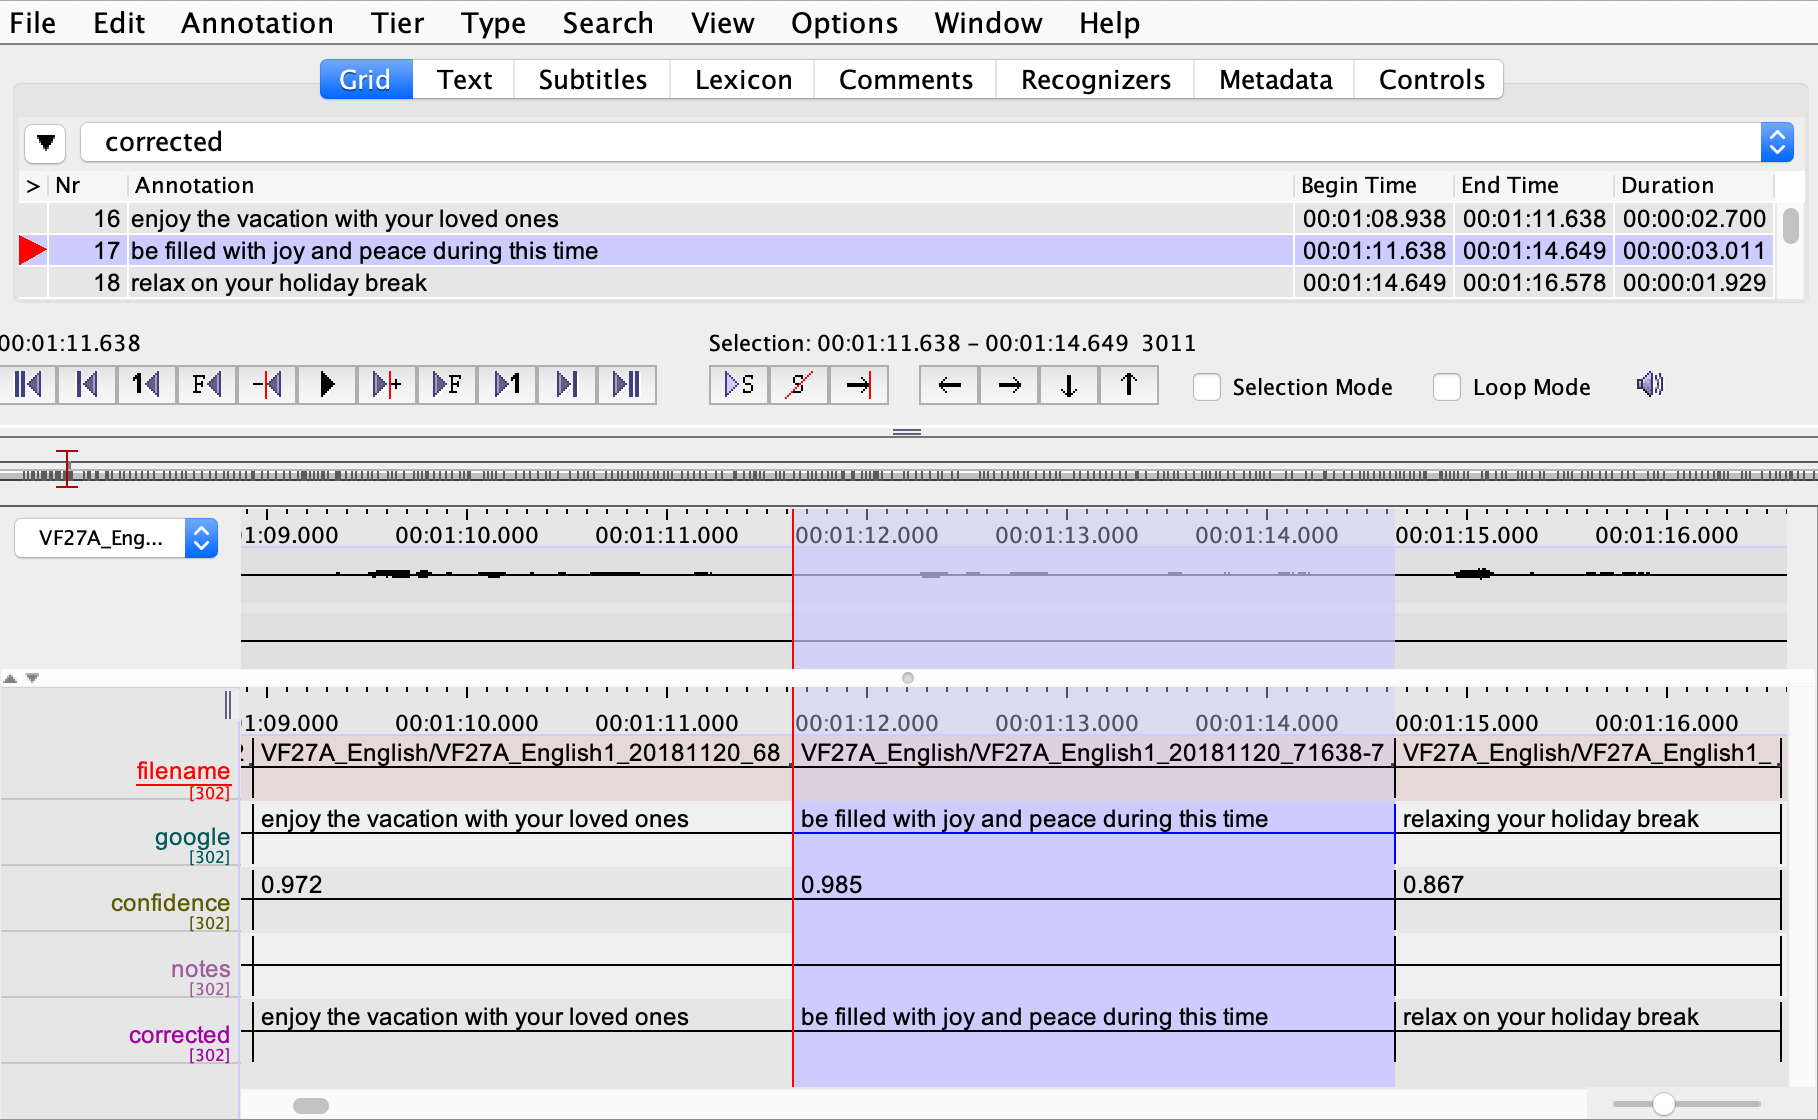
\includegraphics[width=\textwidth]{figures/2-elan_screenshot.png} 
\caption{This screenshot from ELAN showcases a sample of hand-corrected English from the sentence reading task for participant VF27A. The audio waveform is displayed in two channels, with one for the participant (top) and the other for the interviewer (bottom). The annotation tiers include (1) the short audio chunk's filename, (2) the raw speech-to-text transcript, (3) the speech-to-text confidence rating, (4) space for transcriber notes, if any, and (5) the corrected transcript. Note that ``relaxing'' was corrected to ``relax on'' in the rightmost section displayed.}
\label{ch2:fig:elan}
\end{center}
\end{figure*}

\section{Annotation}\label{ch2:sec:annotation}
All recordings were processed according to the pipeline outlined in this section. As much as possible, automatic tools were leveraged to expedite hand correction. 

\subsection{Cloud Speech-to-Text}\label{ch2:subsec:stt}
Google Cloud Speech-to-Text was used to produce an initial transcript of the interviews \citep{google_2019_stt}. This was done using the Short Audio option, with the language variety set to Canadian English (en-CA) or Hong Kong Cantonese (yue-Hant-HK). In order to use this speech recognition product, the participant's speech from the recordings was first segmented into short chunks, typically under 15 seconds in duration.\footnote{The interviewer's speech is included in the recordings for the purpose of context, but is not transcribed.} No attention was paid to constituents at this point; rather, breaks were placed at breaths and other pauses. Short chunks were necessary for speech recognition with locally stored files and desirable for transcribers in the subsequent hand correction phase. With the audio files prepared in this way, speech recognition was completed using the Python client library for Google Cloud Speech-to-Text. The output included both a transcript and a confidence rating for each audio chunk. While the transcripts generated in this fashion were far from perfect, they served the function of expediting the hand-correction process.

\subsection{Orthographic Transcription Hand-Correction}\label{ch2:subsec:orthographic}
The automatically generated transcripts were converted into multi-tiered ELAN transcription files \citep{sloetjes_2008_elan}, with tiers for the automatically generated transcript, phrase transcription confidence, notes, and corrected transcript. During hand-correction, research assistants adjusted the transcript in the corrected tier, and took note of anything pertinent to the given audio chunk. Figure~\ref{ch2:fig:elan} depicts an example of corrected English transcriptions in ELAN \citep{sloetjes_2008_elan}. Direct identifiers (e.g., names) were marked during this phase, and silenced from the recordings prior to release. Transcriber guidelines were adapted from the multilingual Heritage Language Variation and Change corpus, which includes Cantonese \citep{nagy_2011_hlvc}. Guidelines for Cantonese were developed in collaboration with the bilingual research assistant team.

In both languages, the following conventions were used:
\begin{itemize}
 \item The placeholder ``xxx'' denotes unintelligible speech.
 \item Fragments are transcribed using ``\&'' followed by the fragment produced (e.g., ``\&s'').
 \item The ``?'' symbol marks questions; other punctuation is not used.
\end{itemize}

Cantonese-specific conventions include:
\begin{itemize}
 \item Where possible, transcription is in characters.
 \item Words without a standard character are transcribed with Jyutping (e.g., \textit{jyut6ping3}).
%  \item Fully-lexicalized syllable fusion is transcribed with the typical smaller number of characters (e.g., 咩 \textit{me1} is a fully fused version of 乜嘢 \textit{mat1 ye5}, and intermediate version 咩嘢 \textit{me1 ye5}\textemdash all translate to ``what'').\footnote{Syllable fusion is a phenomenon in which adjacent syllables in Cantonese are blended together. It ranges from assimilation at the syllable boundary to segment deletion and re-syllabification \citep{wong_2006_fusion}. Syllable fusion is common in Cantonese, though its frequency of occurrence and degree varies.}
%  \item Non-lexicalized (or ambiguous) cases of syllable fusion are transcribed with the full number of characters fused (e.g., 朝頭早, ``morning,'' is fully pronounced as \textit{ziu1 tau4 zou2}, but can be fused to 【朝頭】早 \textit{ziau14 zou2}. Brackets indicate the fused syllables).
%  \item Filled pauses are transcribed with the character 㖡 (\textit{e6}), or using Jyutping if different (e.g., \textit{m6}). 

 \item Words produced in Mandarin Chinese are transcribed in Mandarin characters with ``@m'' appended to each.\footnote{Most participants report knowledge of Mandarin, though age of acquisition, use, and proficiency all vary drastically. In all cases, Mandarin was learned later than Cantonese and English.}
\end{itemize}

English-specific conventions include:
\begin{itemize}
 \item Standard spelling is used.
 \item Proper nouns are capitalized and hyphenated if composed of multiple words (e.g., ``British-Columbia''). % Decide if I want an RA to go through and clean this up
 \item Filled pauses are transcribed with ``um'', ``er'', ``uh'', and other similar forms.
 \item Numbers are written out in word form (e.g., ``one hundred'').
\end{itemize}

\subsection{Forced Alignment}\label{ch2:subsec:alignment}
Force-aligned transcripts were produced with the Montreal Forced Aligner \citep{mcauliffe_2017_mfa}, using the hand-corrected orthographic transcripts and short audio chunks. 

In Cantonese, forced alignment was completed with the Train-and-Align option, as there was no pretrained model available for Cantonese. The Cantonese pronunciation dictionary was generated using the \textit{PyCantonese} Python library \citep{lee_2018_pycantonese}. As Cantonese orthpgraphy does not separate words with spaces, words segmentation was done according a maximum length matching algorithm... Pronunciations were identified by getting the Jyutping romanization from each character (or using the Jyutping transcribed), separating it into segments, and appending the tone number to the syllable nucleus (i.e., vowel or syllabic nasal). Research assistants supplemented the dictionary with alternative pronunciations for words that participated in syllable fusion. This approach bears some similarity to that of \citet{tse_2019_heritage}, but differs in that it also includes tonal information---which has been shown to improve forced alignment as long as there are not too many tone-nucleus combinations \citep{cavar_2016_endangered, yuan_2014_automatic}. %maybe add a DiCanio reference, see Matt Faytak's email

Forced alignment in English took advantage of the Montreal Forced Aligner's pretrained English model and pronunciation dictionary, which broadly reflects North American English varieties. The dictionary was supplemented with manual additions. 

The force-aligned transcripts were not manually corrected or checked. This means that any short chunk with code-switching or unintelligible speech will likely have poorer alignment. As a result, it is advisable to use stringent exclusionary criteria or perform checks prior to analyzing data from the corpus. 


\section{Descriptive Statistics}\label{ch2:sec:statistics}
As hand-correction is currently underway, the descriptive statistics reported in the section are based on the Google Cloud Speech-to-Text transcripts of all three tasks (sentence reading, storyboard narration, interview) for the 27 participants listed in Table~\ref{ch2:tab:participants}. 

\subsection{Cantonese Interviews}\label{ch2:subsec:cantonese_descriptive}
The Cantonese interviews include approximately 9.43 hours of participant speech.\footnote{Note that this excludes the duration of the interviewer questions, as well as pauses in the participant's speech. Furthermore, with the addition of the remaining seven male participants, this will increase to approximately 12 hours} There were a total of 1,836 character types, and 98,401 character tokens. The number of characters varies somewhat drastically by participant, with a mean of 3,514 characters per interview (SD$=$734, min$=$2,171, max$=$5,410). The overall distribution of character frequency in the Cantonese interviews is depicted in Figure~\ref{ch2:fig:ccf}. As expected, there are a relatively small number of characters occurring frequently (e.g. pronouns, function words, etc.), while a majority are mid and low frequency. 

\begin{figure}[!htbp]
\begin{center}
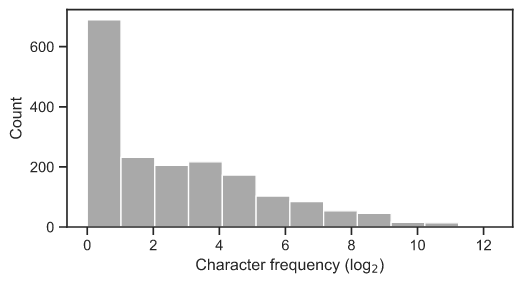
\includegraphics[width=8cm]{figures/2-can_char_frequency.png} 
\caption{The distribution of log character frequency in the Cantonese interviews.}
\label{ch2:fig:ccf}
\end{center}
\end{figure}

The decision to report descriptive statistics for Cantonese in characters rather than words arises from the difficulty of defining wordhood in Cantonese \citep{wong_2006_fusion}, a lack of tools for parsing written Cantonese,\footnote{The \textit{PyCantonese} package is a notable exception to this \citep{lee_2018_pycantonese}, though it does not include tools for splitting sentences into words.} and because written Cantonese does not include spaces between words. An approximation of the word count can be devised by calculating the average word length from the Hong Kong Cantonese Corpus \citep{luke_2015_hkc}\textemdash 1.3 characters. By this estimation, the Cantonese interviews here include approximately 75,115 words.

While Google Cloud Speech-to-Text primarily transcribes Cantonese in characters, it also inserts English text.\footnote{It is unclear at this point how accurate the English text in the Cantonese interviews is, though anecdotally speaking, it is accurate at least some of the time.} As a result, it is possible to get a rough idea of how much code-switching there is in the Cantonese interviews. There were 1,321 English word types in the Cantonese interviews, and 2,858 word tokens. This does not necessarily indicate the number of switches, as participants may have produced more than one English word in a row for a given switch. Nonetheless, it demonstrates that there is a substantial amount of code-switching from Cantonese to English. The mean number of English words in the Cantonese interviews is 102 (s.d.$=$46, min$=$30, max$=$198). 

\subsection{English Interviews}\label{ch2:subsec:english_descriptive}
The English interviews include a total of 5,494 word types and 91,828 word tokens in 9.89 hours of participant speech.\footnote{As with the Cantonese interviews, this will increase to approximately 12 hours with the remaining participants.} As in the Cantonese interviews, the number of words varies substantially by participant, with a mean word count of 3,729 (s.d.$=$701, min$=$2,113, max$=$4,518). The distribution of log word frequency in the English interviews is portrayed in Figure~\ref{ch2:fig:ewf}. Word frequency follows a similar pattern to Cantonese character frequency, with most words occurring infrequently, and a smaller proportion occurring very frequently.

\begin{figure}[!htbp]
\begin{center}
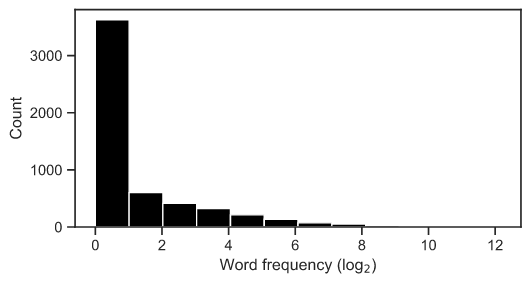
\includegraphics[width=8cm]{figures/2-eng_word_frequency.png} 
\caption{The distribution of log word frequency in the English interviews.}
\label{ch2:fig:ewf}
\end{center}
\end{figure}

Unlike for the Cantonese interviews, it is not possible to get a sense of code-switching in the English interviews, as Google Cloud Speech-to-Text for Canadian English does not insert Cantonese characters. Anecdotally, the interviewers reported that while most of the English interviews contained some code-switches, there was overall less English-to-Cantonese code-switching. This remains to be quantified when the orthographic hand-correction is completed.

\section{SpiCE Corpus Releases}\label{ch2:sec:releases}

The SpiCE corpus will be made publicly available in a series of releases with increasing transcription accuracy and breadth of annotation. The first release is planned for mid-2020, and will include all audio files with accompanying Google Cloud Speech-to-Text transcriptions and a detailed language background questionnaire summary. The second release will include hand-corrected orthographic transcriptions, with force-aligned phonetic transcriptions. These files will be released as they are completed. Further releases will depend on resources, but would likely include phone-level hand correction and/or corrections for a particular subset of phones. All full releases will be described in the online documentation,\footnote{\url{https://spice-corpus.readthedocs.io/}} shared through the LRE Map,\footnote{\url{http://lremap.elra.info}} and announced on the first author's website.

\section{Discussion \& Conclusion}\label{ch2:subsec:discussion}

While various bilingual corpora exist, they lack in different ways. The SpiCE corpus described here enables within-speaker phonetic comparisons across languages. While this would be possible with some of the bilingual speakers in resources like the Bangor corpora \citep{deuchar_2014_corpora}, the recording quality limits the scope of phonetic queries. With the release of SpiCE and its high-quality recordings, scholars have the ability to ask and answer empirically and theoretically motivated research questions within the speech and language sciences using more sophisticated phonetic measurement techniques (e.g., spectral measures, in addition to temporal measures). This offers substantial potential for increasing our understanding of bilingual spoken language from both phonetic and psycholinguistic perspectives. While the recording quality of this corpus offers these particular advantages, SpiCE is also suitable for any other standard corpus-based inquiry with conversational speech, whether linguistic or paralinguistic in nature. The opportunities made available with SpiCE are especially important given the typological difference between the languages under consideration, and the fact that Cantonese is an understudied language. 

\endinput % -------------------------------------------------------- %
